\chapter{Timers}
Before explaining how timers work, let's try to understand why we would need them.

Up until now, when we have wanted events to occur some human-scale time (hundreds or thousands of milliseconds) apart, we have been using long but finite loops to create delays. The loops have been incrementing or decrementing a number in a CPU register many thousands of times; a task which takes an appreciable amount of time to complete. This can be considered a waste of CPU resources. Instead of getting the CPU to do some useful work (controlling a system or monitoring some external signals) it is simply modifying an internal register for a long time. 
Clearly if we could create our delays or periodic events by some other method it would free up our CPU to be able to do other useful things. 
A timer satisfies this need.\\


A timer is a peripheral inside the microcontroller. Essentially it is a configurable hardware counter: a register which \emph{automatically} (without CPU intervention) counts up to a certain value and then starts counting up again from 0. When it reaches the maximum value it triggers an event called an Update Event or Overflow Event which in turn can trigger an interrupt which in turn can get the CPU to jump to executing some specific block of code. We have about 8 different timers on our micro, each with a number. They range from advanced timers to basic timers. The advanced timers have all of the functionality of the basic timers plus a whole lot more functionality for doing fancy things. We will only consider the basic timers in this course as they have the simplest block diagrams and are easiest to understand. 

\section{Basic Block Diagram}
The best way to understand how a timer is implemented and works is to consider the block diagram. The block diagram for the basic timer, timer 6 is shown in \autoref{fig:timer_basic_diagram}.

\begin{figure}
\centering
\includegraphics[page=508, clip=true, trim=195 270 135 430, width=\textwidth]{./stm32f0xx_reference_manual}
% left, bottom, right, top
\caption{Block Diagram of Basic Timer 6. Source: Figure 192, Reference Manual}
\label{fig:timer_basic_diagram}
\end{figure}

\subsection{Clock from RCC}
We know that the timer is centred around a counter which needs to have a well defined frequency. There is a clock line which enters the timer peripheral from the RCC. By default this line is running at 8 MHz. This the TIMxCLK line in the diagram. 

\subsection{Control}
The control block configures how the timer will work. This includes such aspects as:
\begin{itemize}
\item whether the TIMxCLK line is allowed to pass through the control block to the next blocks (counter enabled) or of the TIMxCLK line is prevented from going further (counter disables).
\item whether the timer will generate an interrupt when an overflow even happens
\item whether or not registers are shadowed
\item and many more
\end{itemize}


